\section{SYK models}
%----------------------------------------------------------------------------------------
\subsection{Complex SYK model}
\begin{frame}{Complex SYK model}
\begin{block}{Complex SYK Hamiltonian}
\begin{equation*}
\mathcal{H}_{\mathrm{SYK}} = -\mu\sum_{i} c_{i}^{\dagger} c_{i} + \sum_{i,j,k,l=1}^{N}J_{ijkl} c_{i}^{\dagger} c_{j}^{\dagger} c_{k} c_{l}
\end{equation*}
\vspace{-3mm}
\begin{equation*}
\left\langle J_{ijkl} \right\rangle = 0 \quad \left\langle |J_{ijkl}|^2 \right\rangle = \frac{J^2}{2N^3}
\end{equation*}
\end{block}

% \begin{center}
% Conserved charge: $Q = \sum_i c_{i}^{\dagger} c_{i} - \frac{N}{2}$.
% \end{center}

\qquad Replica trick: $\ln Z = \lim_{n \to 0} \frac{Z^n - 1}{n}$:

\begin{figure}
% \hspace{-1cm}
\begin{minipage}{0.2\linewidth}
% 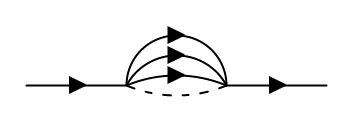
\includegraphics[width=\textwidth]{figs/SYK/FD/1.png}
\feynmandiagram [small, horizontal=f2 to f3] {
        f1 --[fermion]  f2 --[fermion] f3 --[fermion] f4,
        f2 --[fermion, bend right=35] f3,
        f3 --[fermion, bend right=35] f2,
        f3 --[scalar, bend left=90] f2,
    };
\begin{picture}(0,0)
\put(35,0){\text{$\sim n$}}
\end{picture}
\end{minipage}
\hspace{1cm}
\begin{minipage}{0.3\textwidth}
% 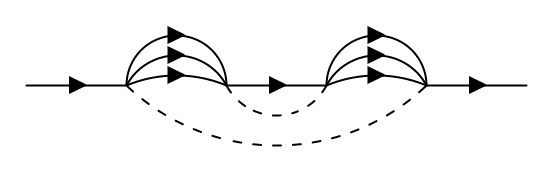
\includegraphics[width=\textwidth]{figs/SYK/FD/2.png}
\feynmandiagram [small, horizontal=f3 to f4] {
        f1 --[fermion]  f2 --[fermion] f3 --[fermion] f4 --[fermion] f5 --[fermion] f6,
        f2 -- [fermion, bend right=35] f3,
        f3 -- [fermion, bend right=35, edge label'=copy a] f2,
        f4 -- [fermion, bend right=35] f5,
        f5 -- [fermion, bend right=35, edge label'=copy a] f4,
        f5 -- [scalar,bend left=90] f2,
        f4 -- [scalar,bend left=90] f3,
    };
\begin{picture}(0,0)
\put(55,10){\text{$\sim \frac{1}{N}$}}
% \put(-45,35){\text{copy a}}
% \put(-85,35){\text{copy a}}
\end{picture}
\end{minipage}
\hspace{1cm}
\begin{minipage}{0.3\textwidth}
% 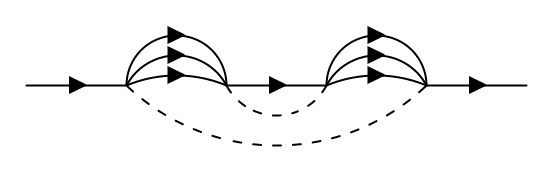
\includegraphics[width=\textwidth]{figs/SYK/FD/2.png}
\feynmandiagram [small, horizontal=f3 to f4] {
        f1 --[fermion]  f2 --[fermion] f3 --[fermion] f4 --[fermion] f5 --[fermion] f6,
        f2 -- [fermion, bend right=35] f3,
        f3 -- [fermion, bend right=35, edge label'=copy a] f2,
        f4 -- [fermion, bend right=35] f5,
        f5 -- [fermion, bend right=35, edge label'=copy b] f4,
        f5 -- [scalar,bend left=90] f2,
        f4 -- [scalar,bend left=90] f3,
    };
\begin{picture}(0,0)
\put(55,10){\text{$\sim n^2$}}
% \put(-45,35){\text{copy b}}
% \put(-85,35){\text{copy a}}
\end{picture}
\end{minipage}
\end{figure}
\end{frame}

\begin{frame}{Dyson equation}
\begin{columns}
\begin{column}{0.5\textwidth}
\begin{figure}
\begin{minipage}{\textwidth}
% 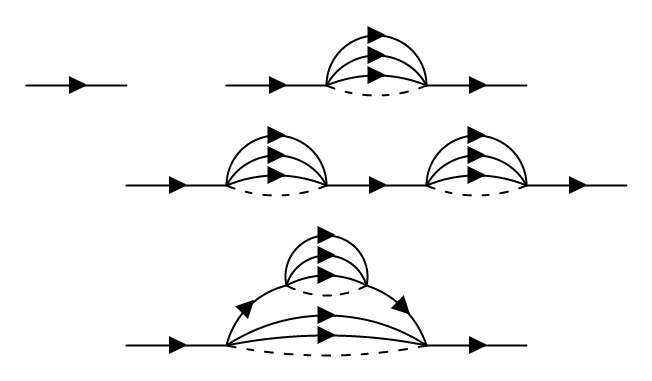
\includegraphics[width=\textwidth]{figs/SYK/FD/G.png}
\begin{equation*}
\begin{aligned}
    &\vcenter{\hbox{\feynmandiagram [small, horizontal=f1 to f3] {
                f1 -- [fermion] f3,
            };}}
    +
    \vcenter{\hbox{\feynmandiagram [small, horizontal=f2 to f3] {
                f1 --[fermion]  f2 --[fermion] f3 --[fermion] f4,
                f2 --[fermion, bend right=35] f3,
                f3 --[fermion, bend right=35] f2,
                f3 --[scalar, bend left=90] f2,
            };}}
    + \\
    &\vcenter{\hbox{\feynmandiagram [small, horizontal=f3 to f4] {
                f1 --[fermion]  f2 --[fermion] f3 --[fermion] f4 --[fermion] f5 --[fermion] f6,
                f2 -- [fermion, bend right=35] f3,
                f3 -- [fermion, bend right=35] f2,
                f4 -- [fermion, bend right=35] f5,
                f5 -- [fermion, bend right=35] f4,
                f3 -- [scalar,bend left=90] f2,
                f5 -- [scalar,bend left=90] f4,
            };}} \\
    &+
    \vcenter{\hbox{\feynmandiagram [small, horizontal=f3 to f4] {
                f1 --[fermion]  f2 --[fermion] f3 --[fermion] f4 --[fermion] f5 --[fermion] f6,
                f2 -- [fermion, bend left=35] f5,
                f5 -- [fermion, bend right=70] f2,
                f3 -- [fermion, bend left=35] f4,
                f4 -- [fermion, bend right=90] f3,
                f5 -- [scalar,bend left=35] f2,
                f4 -- [scalar,bend left=70] f3,
            };}}
\end{aligned}
\end{equation*}
% \begin{picture}(0,0)
% \put(55,109){\text{$+$}}
% \put(20,76){\text{$+$}}
% \put(20,22){\text{$+$}}
% \put(190,22){\text{$+ \quad \cdots$}}
% \end{picture}
\end{minipage}
\end{figure}
\end{column}
\begin{column}{0.5\textwidth}
\qquad When $N \gg 1$:
\begin{center}
% \begin{itemize}
% \item 
Self-consistent Dyson equations:

$$G(i\omega) = \frac{1}{i\omega -\mu - \Sigma(i\omega)}$$

$$\Sigma(\tau_1, \tau_2) = -J^2 G(\tau_1, \tau_2)^2 G(\tau_2, \tau_1)$$

% \item Corresponding action:

% $$\frac{I}{N} = -\ln\det (-\sigma - \Sigma) - \int d\tau_1 d\tau_2 [\Sigma(\tau_1, \tau_2) G(\tau_2, \tau_1) + \frac{J^2}{2} G(\tau_1, \tau_2) G(\tau_2, \tau_1)]$$
% \end{itemize}
%$G(\tau_1, \tau_2) = -\frac{1}{N}\sum_i <Tc_{i}^{\dagger}(\tau_1) c_{i}(\tau_2)>$
%$\sigma = \delta' - \mu \delta$
\end{center}
\end{column}
\end{columns}

Corresponding action:

$$\frac{I}{N} = -\ln\det (-\sigma - \Sigma) - \int d\tau_1 d\tau_2 [\Sigma(\tau_1, \tau_2) G(\tau_2, \tau_1) + \frac{J^2}{2} G(\tau_1, \tau_2) G(\tau_2, \tau_1)]$$

\begin{textblock}{10}(9.5,14.5)
\scriptsize
J. Maldacena et al., PhysRevD.94.106002(2016)
\end{textblock}
\end{frame}
%----------------------------------------------------------------------------------------
\subsection{Supersymmetry Method}
%----------------------------------------------------------------------------------------
\begin{frame}{Supersymmetry Method}

\begin{equation*}
\begin{aligned}
    {\rm Ordinary: }\int _{-\infty }^{\infty }e^{-x^{*}ax}\,dxdx^{*} &= a^{-1} \\
    {\rm Grassmannian: }\int _{-\infty }^{\infty }e^{-\xi^{*}a\xi}\,d\xi d\xi^{*} &= a
\end{aligned}
\end{equation*}

\begin{equation*}
    <O> = \frac{\tr O \exp(-\beta H)}{\tr \exp(-\beta H)} = \tr O_{B,F} \exp(-\beta H_{SUSY})
\end{equation*}

\begin{equation*}
\begin{aligned}
    Z_{\rm SUSY} = \int D\phi^{*} D\phi \exp \{i \int dt [ \sum_{i} \sum_{a=B,F} \phi_{ia}^{*} (i\partial_{t} + \mu) \phi_{ia} - \sum_{ijkl} \sum_{a=BF} J_{ijkl} \phi_{ia}^{*} \phi_{ja}^{*} \phi_{ka} \phi_{la}] \} = 1
\end{aligned}
\end{equation*}

% \begin{equation*}
% \begin{aligned}
%     Z_{\rm SUSY} &= \int D\phi^{*} D\phi \exp \{i \int dt [ \sum_{i} \sum_{a=B,F} \phi_{ia}^{*} (i\partial_{t} + \mu) \phi_{ia} - \sum_{ijkl} \sum_{a=BF} J_{ijkl} \phi_{ia}^{*} \phi_{ja}^{*} \phi_{ka} \phi_{la}] \} \\
%     &= \det(J_{ij;kl}) \int DX D\phi^{*} D\phi \exp \{i \int dt [ \sum_{i} \sum_{a=BF} \phi_{ia}^{*} (i\partial_{t} + \mu) \phi_{ia} \\
%     &+ \sum_{ijkl} \sum_{a,b=B,F} \frac{1}{2} X_{ij}^{ab} J_{ijkl}^{ab} \delta_{ab} X_{kl}^{ab} -i (\phi_{ia}^{*} \phi_{jb}^{*} \delta_{ab} X_{ij}^{ab\dagger} + \phi_{ia} \phi_{jb} \delta_{ab} X_{ij}^{ab}) ] \} \\
%     &= \det(J_{ij;kl}) \int DX D\psi^{\dagger} D\psi \exp \{i \int dt [ \sum_{ijkl} \sum_{a,b=B,F} \frac{1}{2} X_{ij}^{ab} J_{ijkl}^{ab} \delta_{ab} X_{kl}^{ab} + \Psi_j M_{ji} \Psi_i ] \} \\
%     &= \det(J_{ij;kl}) \int DX \prod_{ji} {\rm SDet} M_{ji} \exp \{i \int dt [ \sum_{ijkl} \sum_{a,b=B,F} \frac{1}{2} X_{ij}^{ab} J_{ijkl}^{ab} \delta_{ab} X_{kl}^{ab} ] \} \\
%     &= 1
% \end{aligned}
% \end{equation*}

\end{frame}
%----------------------------------------------------------------------------------------
\begin{frame}{Large $N$ limit}

\begin{equation*}
\begin{aligned}
    \langle \phi_{i{\rm a}}^{*}(t) \phi_{i{\rm b}}(t') \rangle &= \int DQ Q_{i, ab}(t, t') \prod _i {\rm Sdet}Q_i^{-1} \\
    &\quad \exp \{i \int dt dt' \sum_{i} \delta(t - t')(i\partial_{t} + \mu) {\rm Str} Q_i(t, t') \\
    &\quad + i \frac{J^2}{4 N^3} \int dt dt' \sum_{ijkl} {\rm Str} [Q_i(t, t') Q_j(t', t)] {\rm Str} [Q_k(t, t') Q_l(t', t)] \\
    &\quad - {\rm Str} [Q_i(t, t') Q_j(t', t) Q_k(t, t') Q_l(t', t)] \}
\end{aligned}
\end{equation*}

Large $N$ saddle point:
\begin{equation*}
\begin{aligned}
    G(t, t') &= \frac{1}{\delta(t - t') (i \partial_t + \mu) - \Sigma(t, t')} \\
    \Sigma(t, t') &= -2J^2 G(t, t') G(t', t) G(t, t')
\end{aligned}
\end{equation*}
\end{frame}
%----------------------------------------------------------------------------------------
\subsection{Thermodynamic}
%----------------------------------------------------------------------------------------
\begin{frame}{Emergent $\mathbb{SL}(2) \cross \mathbb{U}(1)$ symmetry}
\qquad When $J\tau \gg 1$ or $J\beta \gg 1$:
\begin{itemize}
\item $G(z)=\frac{b}{\sqrt{|z|}}\operatorname{sgn}(z)$: branch cut $\implies$ non-Fermi liquid

\vspace{1cm}

\item Conformal invariance:
\begin{equation*}
\begin{array}{l}
G\left(\tau_{1}, \tau_{2}\right) \rightarrow f^{\prime}\left(\tau_{1}\right)^{\Delta} f^{\prime}\left(\tau_{2}\right)^{\Delta} e^{i\left(\phi\left(\tau_{1}\right)-\phi\left(\tau_{2}\right)\right)} G\left(f\left(\tau_{1}\right), f\left(\tau_{2}\right)\right) \\
\widetilde{\Sigma}\left(\tau_{1}, \tau_{2}\right) \rightarrow f^{\prime}\left(\tau_{1}\right)^{1-\Delta} f^{\prime}\left(\tau_{2}\right)^{1-\Delta} e^{i\left(\phi\left(\tau_{1}\right)-\phi\left(\tau_{2}\right)\right)} \widetilde{\Sigma}\left(f\left(\tau_{1}\right), f\left(\tau_{2}\right)\right)
\end{array}
\end{equation*}

% \begin{equation*}
% \begin{aligned}
% \mathcal{Z} &= \int \mathcal{D} f(\tau) \mathcal{D} \phi(\tau) e^{-N S_{\text {eff }}[f, \phi]} \\
% S_{\mathrm{eff}}[f, \phi] &= \frac{K}{2} \int_0^{1/T} d\tau (\partial_{\tau} \phi + 2i\pi \mathcal{E} T \partial_{\tau} \epsilon)^2 - \frac{\gamma}{4\pi^2}\int_0^{1/T} d\tau \{ \tan(\pi T(\tau + \epsilon(\tau))), \tau \} \\
% \{g, \tau\} &\equiv \frac{g^{\prime \prime \prime}}{g^{\prime}}-\frac{3}{2}\left(\frac{g^{\prime \prime}}{g^{\prime}}\right)^{2}
% \end{aligned}
% \end{equation*}
\end{itemize}

\begin{textblock}{10}(9.5,14)
\scriptsize
R. A. Davison et al., PhysRevB.95.155131(2017)\\
Y. Gu et al., JHEP02(2020)157
\end{textblock}
\end{frame}
%----------------------------------------------------------------------------------------
\begin{frame}{Finite zero temperature entropy}
% \begin{columns}
% \begin{column}{0.5\textwidth}
% \begin{equation*}
% \lim _{\beta \rightarrow \infty} \lim _{N \rightarrow \infty} \frac{S\left(N, Q, \beta \right)}{N}=\mathcal{S}(Q)>0
% \end{equation*}

% \begin{equation*}
% \frac{d \mathcal{S}(Q)}{d Q}=2 \pi \mathcal{E}
% \end{equation*}

\begin{itemize}
    \item Conserved charge: $Q = \frac{1}{N} \sum_i \langle c_i^{\dagger} c_i - \frac{1}{2} \rangle$

    \vspace{0.5cm}
    
    \item Maxwell relation: $(\frac{\partial S}{\partial Q})_T = -(\frac{\partial \mu}{\partial T})_Q$

    \vspace{0.5cm}

    \item $G(z = i \omega_n) = \frac{1}{z} - \frac{\mu}{z^2} + \cdots$ $\implies \mu = - \oint G(z) z dz$

    % \item $\mu = - \oint G(z) z dz = - \lim_{\tau \to 0^+}\partial_{\tau} (G(z) e^{\tau z}) + \lim_{\tau \to 0^-}\partial_{\tau} (G(z) e^{\tau z}) = - \partial_{\tau} G(\tau = 0^+) + \partial_{\tau} G(\tau = 0^-) = - \partial_{\tau} G(\tau = 0^+) - \partial_{\tau} G(\tau = \beta^-)$

    \vspace{0.5cm}

    \item $\frac{d \mathcal{S}(Q)}{d Q}=2 \pi \mathcal{E}$
    
    \vspace{0.5cm}
    
    \item $\lim _{\beta \rightarrow \infty} \lim _{N \rightarrow \infty} \frac{S\left(N, Q, \beta \right)}{N}=\mathcal{S}(Q)>0$
\end{itemize}

% \end{column}


% \begin{column}{0.5\textwidth}
% \begin{tikzpicture}
% \tikzset{box/.style={arrow box, draw=blue}};
% \node[box, arrow box arrows={west:2cm}] at (0,0){\begin{minipage}{8em}Entropy of charged spherical black holes living in asymptotically $AdS_2$ space\end{minipage}};
% \end{tikzpicture}
% \end{column}
% \end{columns}

\begin{textblock}{10}(11,14.5)
\scriptsize
Y. Gu et al., JHEP02(2020)157
\end{textblock}
\end{frame}
%----------------------------------------------------------------------------------------
\subsection{Maximal quantum chaos}
%----------------------------------------------------------------------------------------
\begin{frame}{Spectral density}
\begin{block}{Bohigas-Giannoni-Schmit(BGS) conjecture}
Spectra of systems (with certain discrete symmetry) whose classical analogues are chaotic systems show the same fluctuation properties as predicted by random matrix theory (with the same discrete symmetry).
\end{block}

\vspace{1cm}
\qquad For SYK model:
$$
\begin{aligned}
    \rho(E) = -\frac{1}{\pi} \Im G(w+i0^{+}) &\propto \sinh \left[2 \pi \sqrt{2} \sqrt{\left(1-E / E_{0}\right) /(-\log \eta)}\right] \\
    &\sim \sqrt{\left(1-E / E_{0}\right)}
\end{aligned}
$$
\end{frame}
%----------------------------------------------------------------------------------------
\begin{frame}{Out-of-time-ordered correlator}
\begin{center}
\vspace{-0.5cm}
\begin{equation*}
\begin{aligned}
    F(\tau_1, \tau_2, \tau_3, \tau_4) &= \langle c_i^{\dagger}(\tau_1) c_j(\tau_2) c_i^{\dagger}(\tau_3) c_j(\tau_4) \rangle
    = \sum_n F_n(\tau_1, \tau_2, \tau_3, \tau_4)
\end{aligned}
\end{equation*}

\vspace{-0.5cm}
\begin{equation*}
    F_{n+1}(\tau_1, \tau_2, \tau_3, \tau_4) = \int d\tau d\tau' F_{n}(\tau_1, \tau_2, \tau, \tau') K(\tau, \tau', \tau_3, \tau_4),
\end{equation*}

\vspace{-0.5cm}
\begin{figure}
    \centering
        \begin{equation*}
        \vcenter{\hbox{\feynmandiagram [horizontal=f1 to f3] {
            f1 [particle=\(\tau_1\)] -- fu1 -- [ghost] fu2 -- fu3 -- f3 [particle=\(\tau_3\)],
            f2 [particle=\(\tau_2\)] -- fd1 -- [ghost] fd2 -- fd3 -- f4 [particle=\(\tau_4\)],
            fu1 -- [bend left=30] fd1,
            fu1 -- [bend right=30] fd1,
            fu2 -- [bend left=30] fd2,
            fu2 -- [bend right=30] fd2,
            fu3 -- [bend left=30] fd3,
            fu3 -- [bend right=30] fd3,
        };}}
        =
        \vcenter{\hbox{\feynmandiagram [horizontal=f1 to f3] {
            f1 [particle=\(\tau_1\)] -- fu1 -- [ghost] fu2 -- f3 [particle=\(\tau\)],
            f2 [particle=\(\tau_2\)] -- fd1 -- [ghost] fd2 -- f4 [particle=\(\tau'\)],
            fu1 -- [bend left=30] fd1,
            fu1 -- [bend right=30] fd1,
            fu2 -- [bend left=30] fd2,
            fu2 -- [bend right=30] fd2,
        };}}
        \oplus
        \vcenter{\hbox{\feynmandiagram [horizontal=f1 to f3] {
            p [particle=\(\tau\)] -- [draw=none] fu3 -- f3 [particle=\(\tau_3\)],
            p' [particle=\(\tau'\)] -- [draw=none] fd3 -- f4 [particle=\(\tau_4\)],
            fu3 -- [bend left=30] fd3,
            fu3 -- [bend right=30] fd3,
        };}}
    \end{equation*}
\end{figure}

\vspace{-0.5cm}
Out-of-time-ordered correlator(OTOC): $\frac{1}{N} \sum_i \langle c_{i}^{\dagger}(\tau) c_{i}(0) c_{i}^{\dagger}(\tau) c_{i}(0) \rangle = f_{0} - \frac{f}{N} e^{\frac{2\pi}{\beta} \tau}$% where  $\lambda_{\mathrm{SYK}} = \frac{2\pi}{\beta}$ for SYK model

% \vspace{1cm}
MSS bound: exponential exponent $\lambda \le \frac{2\pi}{\beta}$

% \vspace{1cm}
% For SYK model $\lambda_{\mathrm{SYK}} = \frac{2\pi}{\beta}$
\end{center}

\begin{textblock}{10}(10.5,14.5)
\scriptsize
J. Maldacena et. al., JHEP08(2016)106
\end{textblock}
\end{frame}
%----------------------------------------------------------------------------------------

%----------------------------------------------------------------------------------------
\subsection{Duality to $AdS_2$ black hole}
%----------------------------------------------------------------------------------------
\begin{frame}{Duality}

\begin{table}[]
\centering
\begin{tabular}{|c|cc|}
\hline
 &
  \multicolumn{1}{c|}{SYK model} &
  \begin{tabular}[c]{@{}c@{}}a $U(1)$ charged Einstein-Maxwell\\ gravity in AdS$_2$ space\end{tabular} \\ \hline
$S = -C \int dt \{ f(t), t) \}$ &
  \multicolumn{1}{c|}{\begin{tabular}[c]{@{}c@{}}Ghost coming from\\ the conformal symmetry\end{tabular}} &
  Boundary gravitons \\ \hline
$\frac{\partial S_{\rm BH}}{\partial Q} = 2\pi \mathcal{E}$ & \multicolumn{2}{c|}{Same finite entropy relation} \\ \hline
$\lambda = \frac{2\pi}{\beta}$                              & \multicolumn{2}{c|}{Maximum quantum chaos}        \\ \hline
\end{tabular}
\end{table}

\end{frame}